    \section{\label{sec:attack-recipe}Integration of an existing attack}
        The tool was designed to be extensible, allowing the users to create, include and test their own attacks. Integrating a new existing attack consists of several steps. It will be easiest to present the individual steps on an example attack. The example is not a real attack and for the demonstration purposes it will not be elaborate. However, it should give the reader enough information for integrating her custom attack. Roughly, we will cover the following steps:

        \begin{itemize}
            \item adding the attack source files to the framework,
            \item building and compiling the attack source code,
            \item configuring the build,
            \item defining the attack scenario (and adding a custom stage),
            \item registering the attack,
            \item validating the attack.
        \end{itemize}

        The following subsections are discussing the \texttt{example_attack} attack, that reader can find in the project repository in \filepath{javus/data/attacks/example_attack}, if the reader would wish to see the details. The rest of the filepaths in this section are relative to the \texttt{example_attack} directory.% TODO link to appendix.
        % FIXME refernce appendix

        \subsection{Adding the attack source files to the framework}\label{subsec:recipe:add:sources}

        The \texttt{example_attack} consists of one JavaCard source file \filepath{src/com/ExampleAttack.java} (the contents can be viewed in~\ref{section:adding:attack:sources}), which implements a single JavaCard applet. The applet accepts the following instructions:

            \begin{enumerate}[align=left]
                \item[\mintinline{java}{INS_PREPARE}] simulates sending APDU command, that prepares the attack applet, for example, it can return some address values, that will be needed later,
                \item[\mintinline{java}{INS_ATTACK}] simulates the instruction, that will attempt to retrieve some secret data, e.g.\ a secret keys residing somewhere in the non-volatile memory.
            \end{enumerate}
            
            In general the attack can be more complicated, comprisig of multiple applets (and packages) and can implement as many instructions as needed. The sources files should all be under the directory \filepath{javus/data/attacks/<attack-name>}. The \texttt{<attack-name>} must be a valid Python identifier\footnotemark.
            \footnotetext{In practice this might not introduce much of a difference to common directory naming practices \texttt{<attack-name>}. Most notable dots and dashes cannot be used and the \texttt{<attack-name>} cannot start with a digit.}
            In Appendix~\ref{subsec:newskeleton} and example boostraping with the utility \javusdev is shown.


    \subsection{Building and compiling the source code}\label{subsec:build:compile}
        % FIXME add some text here.

            \subsubsection{Ant build targets}\label{subsubsec:ant-targets}
            Building the source files is an elaborate process, that must follow certain rules to allow the framework to build the attack dynamically during the runtime of the analysis. To build the sources we use Apache Ant, \texttt{ant-javacard} and \texttt{oracle_javacard_sdks} (see the list of tools used~\ref{subsec:3rd-party} for more information). The framework expects the file \mintinline{bash}{build.xml} in the attack directory and requires the following Ant targets to be implemented:

            % To allow the framework to build the sources dynamically during the runtime of the analysis we need to add \mintinline{bash}{build.xml} file which must implement the following targets:
                \begin{enumerate}[align=left]
                    \item[\mintinline{bash}{build-version}] builds a single version of the attack (e.g. \mintinline{bash}{jc222} for JC SDK 2.2.2.), needs the \mintinline{bash}{version} property defined,
                        % needs the \mintinline{bash}{-Dversion=<sdk_version>} definition to specify, which JavaCard SDK to use to build the applets for the attack
                    \item[\mintinline{bash}{build-all-versions}] does not need any properties as it will build the attack for all SDK versions defined in \mintinline{bash}{config.ini}, 
                    \item[\mintinline{bash}{clean-version}] removes the build files for a particular version, needs the \mintinline{bash}{version} property defined,
                        % needs the \mintinline{bash}{-Dversion=<sdk_version>} definition to specify, for which JavaCard SDK version it should clean the build files,
                    \item[\mintinline{bash}{clean-all-versions}]  does not need any properties as it should clean build files for all the JC SDK versions.
                \end{enumerate}

            \subsubsection{The build configuration}
                A part of the configuration is kept in two separate files \mintinline{bash}{config.ini} and \mintinline{bash}{aids.ini}. This configuration is kept outside of the file \mintinline{bash}{build.xml}, because both Ant and the framework need to interact with them. Both configuration files have to contain the \mintinline{bash}{[BUILD]} section. The \mintinline{bash}{config.ini} then has to set those values:
                \begin{enumerate}[align=left]
                    \item[\mintinline{bash}{versions}] defines a comma separted list of SDK versions, for which the attack is implemented e.g. \mintinline{bash}{"jc222,jc303"},
                    \item[\mintinline{bash}{unsupported.versions}] is optional (comma separated list) and defines the SDKs, that are not supported.
                \end{enumerate}

                Custom configuration values can be added here or directly to \mintinline{bash}{build.xml}. The \mintinline{bash}{aids.ini} is part of the solution of overcoming the problem of unique AIDs (see~\ref{sec:uniq-aid}). In this file the user should define the AIDs for all the applets and packages in this attack. Because \mintinline{python}{example_attack} only installs one applet we can follow the default configuration for \mintinline{bash}{aids.ini} and define the AID as:
                \begin{enumerate}[align=left]
                    \item[\mintinline{bash}{pkg.rid}] sets the RID value for the package \mintinline{bash}{com.examplepackage},
                    \item[\mintinline{bash}{applet.pix}] sets the PIX value for the applet \mintinline[breaklines,breakafter=.]{python}{com.examplepackage.ExampleAttack}.
                \end{enumerate}

                The applet AID will be then concatenated from the values \mintinline{bash}{pkg.rid} and \mintinline{bash}{applet.rid}. In case \javus finds there is an AID match, the value \mintinline{bash}{pkg.rid} will be incremented until there is no collision.

                However, it is more probable, that we will need to set those values for more than one applet. In that case we can update the \mintinline{bash}{build.xml} and \mintinline{bash}{aids.ini} as we wish, but the framework needs to know, how to make the values defined in \mintinline{bash}{aids.ini} unique. For that we need to add a new class called \mintinline{python}{AttackBuilder} to the module file \examplemodule, which will inherit from \shortbuilderclass (see~\ref{subsec:builder-class}). On this class we need to implement \mintinline{python}{uniq_aids} and \mintinline{python}{uniqfy} methods. Both those methods have access to the values defined in \mintinline{bash}{aids.ini} through the dictionary \mintinline{python}{self.aids["BUILD"]} and accept \mintinline{python}{used} parameter, which is a list of AIDs, that are installed on the card at a particular time (before this attack is executed) during the runtime. The purpose of these methods is the following:
                \begin{enumerate}[align=left]
                    \item[\mintinline{python}{uniq_aids(self, used) -> bool}] should return \mintinline{python}{True}, if the AIDs, that this attack defines are \textbf{not} intersecting the AIDs in the list \mintinline{python}{used}, and \mintinline{python}{False} otherwise,
                    \item[\mintinline{python}{uniqfy(self, used) -> None}] is called in case the previous method returns \mintinline{python}{False}. Then it needs to update \mintinline{python}{self.aids["BUILD"]} dictionary, until \mintinline{python}{uniq_aids} returns \mintinline{python}{True}.
                \end{enumerate}

                % In case the reader finds the problem with uniqueness of AIDs bit harder to grasp we advice him to read through the appendix~\ref{section:appendix:new-attack}, where those concepts are discussed further. The next section explains how to define the scenario for ExapmleAttack.

                \subsection{The definition of an attack scenario}\label{subsec:scenario:definition}
                Each attack must define its own scenario in its module file, i.e. \examplemodule for the \texttt{example_attack}. The scenario stages are items of a class level list \mintinline{python}{Scenario.STAGES} in the Python module file. The stages for \texttt{example_attack} are defined in the listing~\ref{lst:scenario:stages}. Each stage is defined as a Python dictionary and must contain the key \mintinline{python}{"name"}, which is used to locate the correct method during runtime. Each stage can be \mintinline{python}{"optional"} (the attack execution continues no matter stage's result) and have a \mintinline{python}{"comment"} that will be saved alongside the stage results. Furthermore, the \install stage requires the \mintinline{python}{"path"} key, that sets the path to the CAP file, that will be installed (its substring \mintinline{python}{{version}} gets formatted to a particular SDK version during the runtime). The path is relative to the attack directory. The \send stage requires the \mintinline{python}{"payload"} key defined with the APDU command (the example scenario definition can be see in Appendix~\ref{sec:definition:of:scenario}).

    The only piece left is how the framework knows, to which applet is it supposed to send the APDUs from the \send stages. For now, the framework can send APDUs only to one applet per each attack. This limitation can be extended, but was not needed for neither of the attacks currently implemented. The framework needs to know, how to create the AID from the values in \mintinline{bash}{aids.ini}, this is implemented in the method \mintinline{python}{construct_aid(self) -> bytes} on the \attackbuilder class. % FIXME

        % Because each attack has a different scenario we need to define it for every attack.
        % To make it simple, yet extensible in the future we have decided to put a Python module into the directory of every attack. %TODO the name of the module should be probably change to scenario.py


% class Stages:
%     STAGES = [
%         {
%             "name": "install",
%             "path": "build/{version}/malicious.cap",
%             "comment": "custom malicious applet",
%             "optional": False,
%         },
%         {
%             "name": "send",
%             "payload": "0x80 0x02 0x00 0x00 0x02",
%             "comment": "read out the secret memory",
%             "optional": True,
%         },
%     ]
    The stages are executed in the order they are defined. The diagram in~\ref{fig:execute-scenario} shows the execution of the scenario. It is worth noting, that we don't need to hardcode the stages' definitions. We can make use of Python and build the stages dynamically. For example this is done in the definition of TransactionConfusion attack scenario.

        \begin{figure}[htb!]
            \centering
            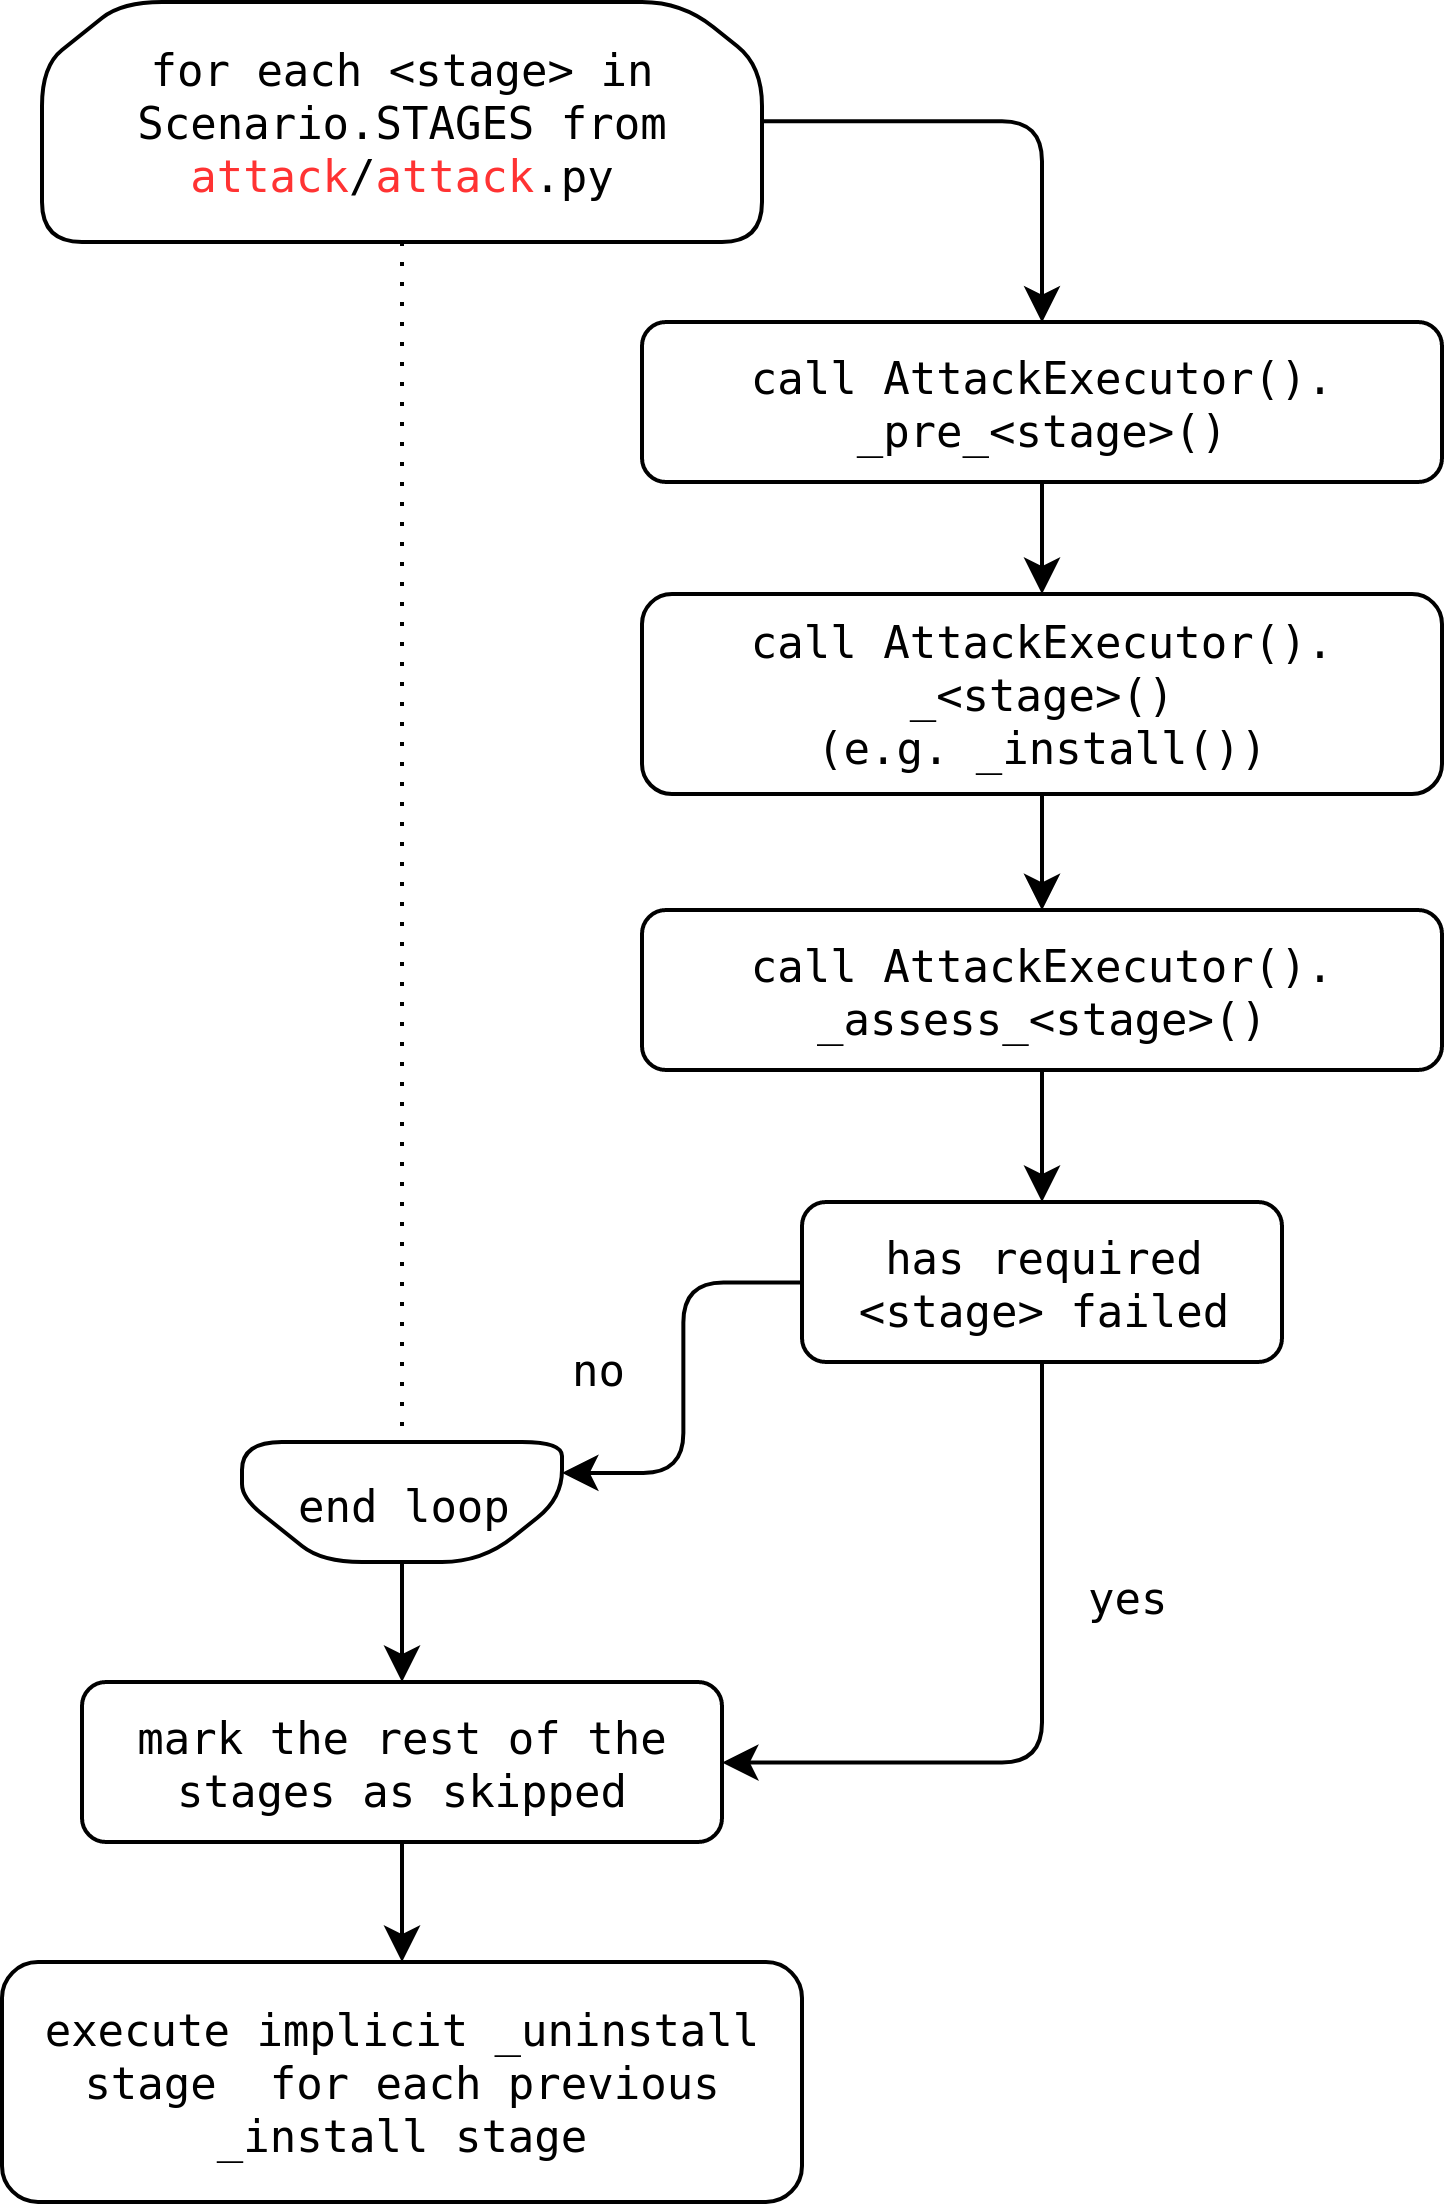
\includegraphics[width=0.7\textwidth]{src/diagrams/execute-scenario.png}
            \caption{Control flow graph explaining the order of execution of different stage methods.}
            \label{fig:execute-scenario}
        \end{figure}

            % \subsection{The common stages}\label{subsec:common-stages}
            %     As we mentioned in~\ref{subsec:executor:class} the common attack stages are (un)installation of CAP files and sending APDU commands. Internally those are implemented as methods on the \shortexecutorclass class. 

                % Due to the way JavaCard environment is build, it is only natural, that multiple attacks have similar structure --- installation, sending APDU commands and uninstallation. The JavaCard Vulnerability Scanner framework comes with those three stages already implemented, but the user of the application can easily extend it with their own (we will explain how to do so later). Internally as seen from the JavaCard Vulnerability Scanner framework point of view each stages is a Python function (or rather method, as it is a class funcion). As such it receives certain parameters and returns a value. Now we will go through the stages already implemented by JavaCard Vulnerability Scanner.

        % \subsubsection{install}
        %     As apparent from the name, this stage is used for installing packages and applets. This stage can install only one CAP file at a time, but can use this stage multiple times within one scenario. The parameters for this stage are listed in~\ref{fig:stage-install-params}.
            % \begin{figure}[h!]
            % \begin{enumerate}[align=left]
            %     \item[name] 
            %     \item[path]
            %     \item[comment]
            %     \item[optional]
            % \end{enumerate}
            % \end{figure}
            % "name": "install",
        %     "path": "build/{version}/com/se/vulns/javacard/vulns.new.cap",
        %     "comment": "The altered vulnerable applet",
        %     # install should be required by default
        %     "optional": False,
        % \subsubsection{send}
        % {
        %     "name": "send",
        %     "payload": "0x80 0x10 0x01 0x02	0x04	0x00 0x00 0xc0 0x00				0x7F",
        %     "comment": "read memory",
        %     "optional": True,
        % },
        % \subsubsection{uninstall}



    % Now that we have defined some terms we can look at some of them in greater detail.

            
    
    % TODO what with thiss
    % After discussing the ins and outs of the logical attack against the JavaCard platform we will explain the design of the testing tool \javus. Few key points need to be stressed. It is a prototype.
        % \subsection{Defining stages}
        % Now that we have means how to build and rebuild the attack during the runtime we can move on to defining the scenario and it's stages. The stages need to be defined in the module file \mintinline{python}{example_attack.py}.



    \subsubsection{Custom stage definition}\label{subsubsec:custom-stage}
    In case the default stages are not covering a particular step in the attack scenario we can add a custom stage. Let us call it \mintinline{python}{foobar}. Similarly to the default stages we will add the \mintinline{python}{foobar} stage to the \mintinline{python}{Scenario.STAGES} list. However, because it is a custom stage we need to also implement it. We must at least define the methods \mintinline{python}{_foobar}, that implements the main stage logic and \mintinline{python}{_assess_foobar}, which must accept the dictionary parameter \mintinline{python}{result} and populate its \mintinline{python}{"success"} key with either \mintinline{python}{True} or \mintinline{python}{False} value. We can also implemnent the \mintinline{python}{_pre_foobar} method and do any setup needed for the stage. All these methods are defined on the \attackexecutor class, that subclasses \shortexecutorclass (if it is not clear where to place this class see~\ref{subsec:executor:class}).



        All of the \mintinline{python}{"<key>": "<value>"} pairs except the \mintinline{python}{"name"} from the stage definition are passed as keyword arguments to the stage methods. Therefore the stage methods need to accept them (we can also make use of the \mintinline{python}{*args, **kwargs} Python syntax to accepts \textit{any} arguments). The example code is in the Appendix in listing~\ref{lst:new:stage}. The \mintinline{python}{AnalysisManager} will attempt to save the complete contents of \mintinline{python}{result} dictionary from the listing~\ref{lst:new:stage} to the database. However, only Python values, that can be encoded as BSON with Python \mintinline{python}{bson} module will be saved.

    \subsection{Registering the attack}
    As of now, the only way to add a new attack is to work in the structure of the Git project --- it's not possible to register an attack, that is outside of the project directory tree. Therefore, make sure, that the attack (in our case \texttt{example_attack}) files reside in the directory \filepath{javus/data/attacks/example_attack}.

    The last thing needed for the attack to be executed by the framework is to add a line to the file \filepath{javus/data/registry.ini}. This file follows a simple structure. Attacks are grouped by sections (e.g.\ the attacks from Security Explorations are in the section \mintinline[breaklines,breakbefore=E]{python}{[SECURITY EXPLORATIONS]}). The user picks an appropriate section or add a new one and add a new line entry saying \mintinline{ini}{example_attack = yes} (if the user wants to let the framework know about the attack, but disable it for now from the analysis set the value to \mintinline{ini}{no}). The user can verify, that the attack is registered by running \mintinline{bash}{javus list}. The user should see his attack in the output.

    \subsection{Validating the attack}
    To help the user with adding a new attack we have also implemented a \mintinline{python}{validate} sub command for the script \javus. \mintinline[breaklines]{python}{javus validate --attack <attack-name>} will validate the \texttt{<attack-name>}. Stage execution can not be easily validated, so the user should be careful.
    % is provided then only the \mintinline{bash}{<attack-name} attack is validated. However, not everything about the attack can be validated (e.g.\ saving custom results of custom stages) so the user might need to be cautious.
